\documentclass[a4paper]{article}
\usepackage{estilo}
\title{\vspace{-1.5cm}Taller \LaTeX}
\author{Rafael Jurado Ariza}
\date{\today}
\begin{document}
    \maketitle
    Hola esto es una ecuación en línea con el texto $1+1=2$.\\
    Esto es una ecuación numerada:
    \begin{equation} 
        1+1=2
    \end{equation}
    Esto es una ecuación sin numerar:
    \begin{equation*}
        E_1=mc^2 
    \end{equation*}
    
    Esto es una ecuación en varias líneas:
    \begin{align*}
        2+2&=6-2\\
        &=4=\frac{12}{3}
    \end{align*}
    Corchetes y paréntesis automáticos: 
    \begin{equation*}  
        \left(1+1=2=\frac{4}{2}\right) 
    \end{equation*}
    Letras griegas:
    \begin{equation*}
        \lambda,\alpha,\psi,\omega
    \end{equation*}
    \begin{figure}[h!]
        \centering
        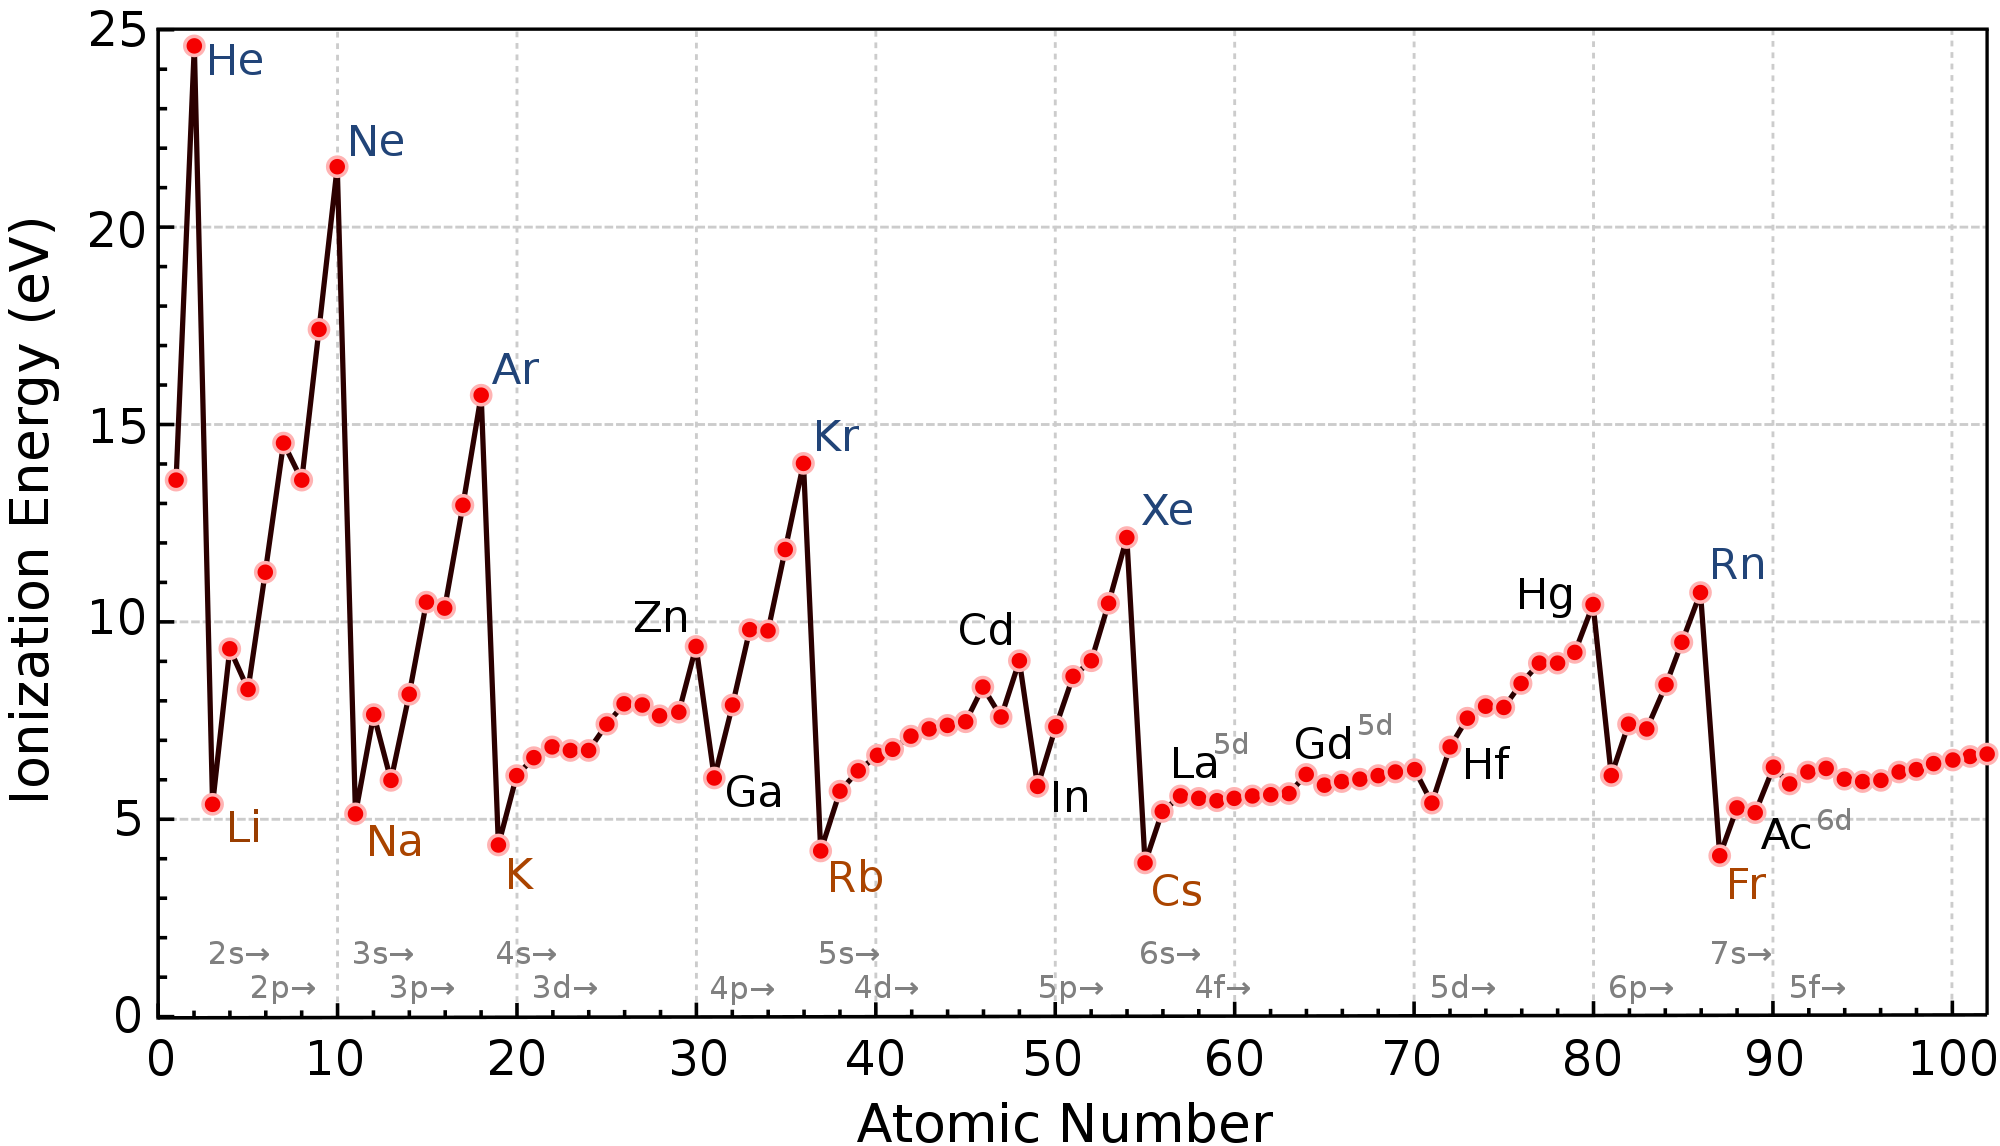
\includegraphics[scale=0.18]{pic/Ionization_energies.png}
        \caption{Esto es un taller}
        \label{fig:energy}
    \end{figure}
    \newpage 
    Esto es la figura \ref{fig:energy}
\end{document}
